\chapter{Metode og proces}

I dette kapitel er der beskrevet kort, hvilken analyse- og designmetode der er anvendt i bachelorprojektet. 

\section{Analyse og designmetode}

Dette afsnit har til formål at beskrive, hvilke tekniske metoder, der er benyttet af udarbejdelsen af bachelorprojektet. Primært er der tale om metoder fra faget ISE. Desuden beskæftiger afsnittet sig med, hvilke arbejdsredskabe, der er anvendt til udførelse af bachelorprojektet og rapporten.

Projektforløbet er organiseret efter V-modellen og ASE-modellen, se figurene \ref{fig:vmodel} og \ref{fig:asemodel}. ASE-modellen anvendes til udvikling af software og hardware, som er delt op i faser. For hver fase kommer en række artefakter som tilsammen resulterer i et dokumenteret bachelorprojekt. Disse faser kombineres med V-modellen. I dette bachelorprojekt er der udført modultest på alle moduler i både hardware og software. Efter godkendelse af modultestene, er en integrationstest blevet udført, hvor det bygget hardware og software er sammensat og testet som et samlet system. Her observeres om systemet fungerer efter hensigten inden accepttesten påbegyndes. Accepttesten undersøger om alle krav specificeret i kravspecifikationen er opfyldt. Vejleder, Thomas Nielsen, Adjunkt på Institut for Ingeniørvidenskab på Aarhus Universitet. har deltaget i udførelsen af accepttesten, godkendt. Bivejlederen Samuel Alberg Thrysøe, Associate Professor PhD ved Ingeniørhøjskolen Aarhus Universitet har fulgt accepttestens udførelse ved sidelinjen.  

\begin{figure}[H]
\centering
{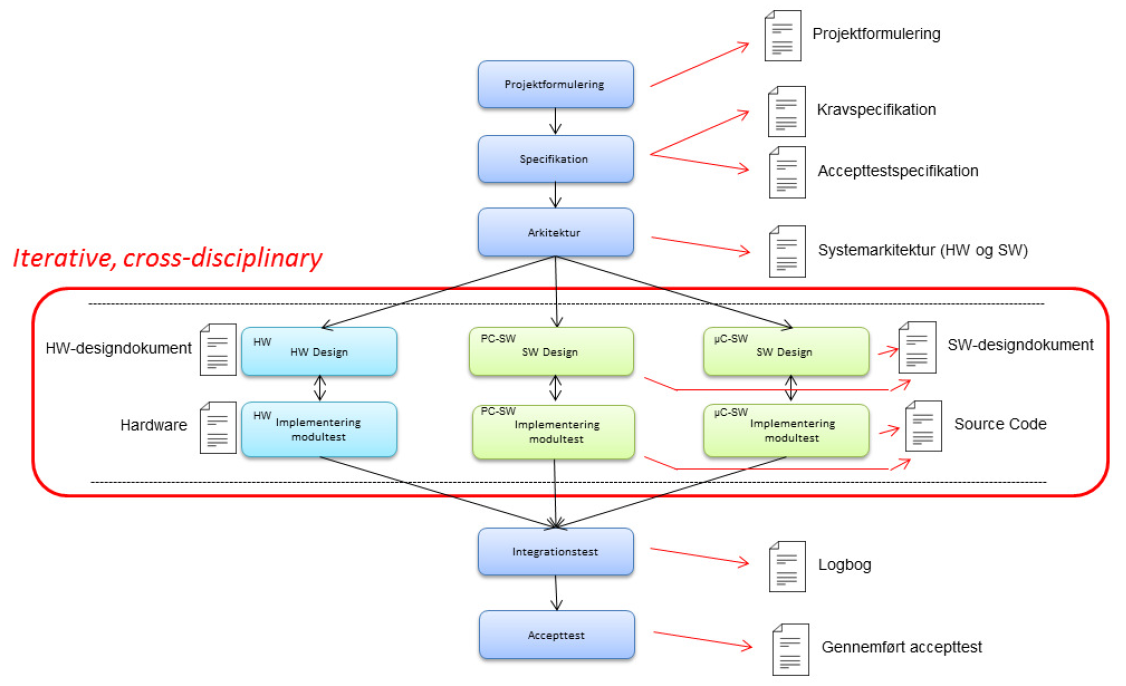
\includegraphics[width=12cm]
{Figure/asemodel}}
\caption{ASE-modellen som er udviklet af Aarhus Ingeniørskole\cite{IngeniorhojskolenAarhusUniversiteta}.}
\label{fig:asemodel}
\end{figure}

\begin{figure}[H]
\centering
{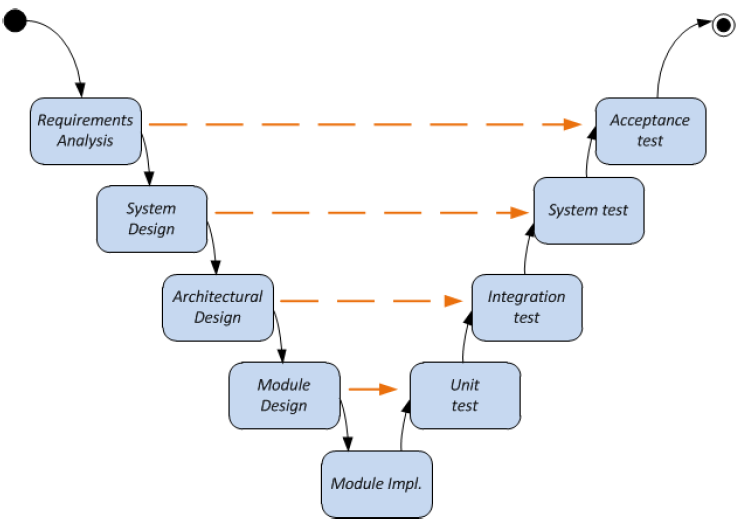
\includegraphics[width=10cm]
{Figure/vmodel}}
\caption{V-modellens udviklingsfaser\cite{IngeniorhojskolenAarhusUniversiteta}}
\label{fig:vmodel}
\end{figure}

ASE-modellen mangler en analysefase som er nødvendigt dette projekt. Derfor besluttede gruppen at modificere ASE-modellen således at den imødekommer dette projekts behov. Modificeringen omfatter en ekstra fase der tilføjes i mellem specifikationens- og arkitekturfasen, se figur \ref{fig:procesVoresASE}.


\begin{figure}[H]
\centering
{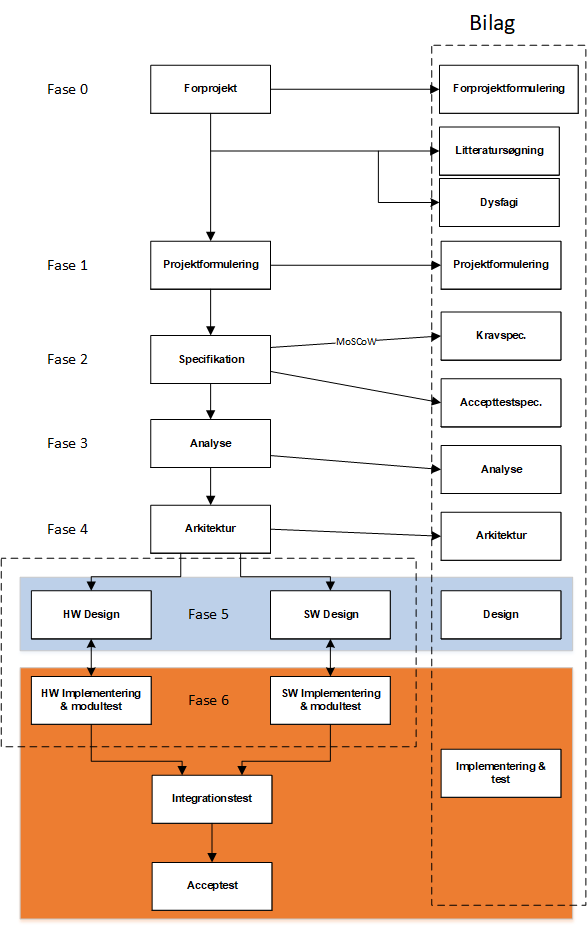
\includegraphics[width=10cm]
{Figure/procesVoresASE}}
\caption{Den modificeret ASE-model.}
\label{fig:procesVoresASE}
\end{figure}

Bachelorprojektets udvikling  er inddelt i forskellige faser mellem nul til seks.

\textbf{Fase 0}\\
Fase nul består af et forprojekt, hvor der blev udarbejdet en projektformulering på baggrund af en udleveret projektbeskrivelse og i samarbejde med vejleder. Her blev der udarbejdet et udkast af kravspecifikationen og en projektplan. Disse kan ses i \nameref{bilag10}.

\textbf{Fase 1}\\
Denne fase bliver brugt til at finde litteratur om emnet dysfagi og hvordan man kan udvikle en prisbillig BI-sensor til at detektere synk. Der blev søgt primærlitteratur i f.eks. databaserne Embase og Pubmed. Derudover er der suppleret den primærlitteratur med sekundærlitteratur i form af lærebøger. Søgeprotokollen til den primærlitteratur kan ses i \nameref{bilag12}.

\textbf{Fase 2}\\
I fase to blev MoSCoW kravene til produktet nedfældet på baggrund af projektformuleringen. Disse er samlet i dokumenterne kravspecifikation og acceptestspecifikation. Dokumenterne kan læses i \nameref{bilag1} og \nameref{bilag2}.

\textbf{Fase 3}\\
Den tredje fase indeholder analysefasen. Første del af analysefasen består af at realisere og teste et kendt kredsløb fra artiklen \textit{"Bioimpedance Analysis: A Guide to Simple Design and Implementation"}. Test og undersøgelser af denne fase blev til dokumentet Analyse, hvilken kan ses i \nameref{bilag3}.

\textbf{Fase 4}\\
I den fjerde fase blev arkitekturen til software og hardware beskrevet. Arkitekturen blev dokumenteret ved hjælp af sysML, hvor BDD og IBD diagrammer blev oprettet. Arkitekturen kan læses i \nameref{bilag4}.

\textbf{Fase 5}\\
I designfasen blev software og hardware designet. Hardwaren blev dokumenteret med diagrammer, udregninger og styklister. Software blev dokumenteret med funktions beskrivelser, et sekvensdiagram og et UML-aktivitetsdiagram. Detaljerne kan læses i \nameref{bilag5}.

\textbf{Fase 6}\\
Til sidst i den sjette fase blev software og hardware implementeret, modultestet og samlet til en integrationstest. Til slut blev accepttesten udført. Yderligere detaljer om denne fase er henvises der til \nameref{bilag6}.

\section{Den gennemførte proces}


\textbf{Gruppedannelse}\\
Gruppen består af to sundhedsteknologistuderende, der er dannet udefra en fælles interesse for projektets beskrivelse. Begge gruppemedlemmer har inden valget af projektet, talt sammen om en mulig gruppedannelse, hvis der kommer et projekt, hvor begge medlemmer finder det interessant. Det kan siges at gruppen er dannet udefra interessen for projektets indhold og en kendskab til hinanden i forvejen. 

\textbf{Samarbejdsaftale}\\
I dette bachelorprojekt er der genanvendt en samarbejdsaftale fra tidligere semestre med få ændringer. Denne samarbejdsaftale kan læses i \nameref{bilag7}. Her er der beskrevet i bestemte punkter, hvordan gruppen skal arbejde og skal forholde sig under hvert punkt. Den blev godkendt og underskrevet af alle gruppens medlemmer. Udbyttet af at anvende samarbejdsaftalen var positivt for gruppen. Især det benyttet ugeskema gjorde, at man kunne administrere sin tid bedre med fag udover bachelorprojektet. 
\pagebreak
\textbf{Arbejdsfordeling}\\
Arbejdsbyrden var ligeligt fordelt i mellem gruppemedlemmerne. Hvor den generelle rapportskrivning af afsnit blev tildelt efter, hvem der havde tid og hvad der var bedst for bachelorprojektet. Administrationen af opgaver blev oprettet og styret fra online portalen Pivotal Tracker, som er et Scrum værktøj. Her blev der i fællesskab oprettet opgaver efter pointsystem om hvor vigtig opgaven var. Det var så muligt at tage opgaver og udføre dem, indenfor for et sprint på en uge. Efter en uge ville man kunne få et overblik over afsluttede opgaver i det pågældende sprint. En nærmere beskrivelse og brugen af Pivotal Tracker findes i \nameref{bilag16}.

\textbf{Planlægning}\\
I den overordnet planlægning blev der bruget online portalen Teamgantt. Her blev der oprettet en kalender over hele forløbet delt op i forskellige faser fra ASE-modellen. Denne kalender havde hele gruppen adgang til og mulighed for at opdatere projektets tidsplan. Gruppens brug af Teamgantt og indstillinger kan læses nærmere i \nameref{bilag16}. For at opretholde en historik over tidsplanen blev der oprettet en versions historik af tidsplanen, denne kan ses i \nameref{bilag17}.

Det daglige arbejde blev nedskrevet i logbogen ved dagens afslutning. Logbogen blev også brugt til at notere beslutninger, ændringer og større arbejde ifm. projektet. For at læse den komplette logbog se \nameref{bilag14}.

\textbf{Møder}\\
For at opretholde overblikket og en fast struktur i projektet var der faste møder i gruppen. Hver morgen startet med scrum møde, hvor hver gruppemedlem præcenteret igangværende opgaver og problematikker. Hver fredag blev der holdt et møde der evaluere ugens arbejde. En gang om ugen var der vejledermøde med en faste dagsordenspunkter samt varierende punkter. Alle møder kan læses i \nameref{bilag18}.

\textbf{Projektledelse}\\
I dette bachelorprojekt var der valgt ikke at have en projektleder. Der var i stedet valgt en kollektiv ledelsesstil. Det har gjort at hele gruppen har skulle have overblik i hele projektet. Samtidig har det været med til at alle i gruppen kender målet og retningen og der er tydelige kommunikation og opfølgninger med faste møder og scrum møder hver dag. Den fælles ledelsesstil har gjort at alle deltagere er engageret og hele tiden kender målet og er klar til at ændre sådan, at målet opnås på den bedste mulige måde. Da der er mange praktiske opgaver i bachelorprojekt, er der lavet en rollefordeling igennem hele projektet. De specifikke roller kan ses i \nameref{bilag7}.

\textbf{Projektadministration}\\
Rapporten og bilag er skrevet i tekstsproget \LaTeX. Møder, referater og logbog er skrevet i Google Docs. Tidsplan og opgaver er oprettet og ligger i selvstændige online værktøjer: Teamgantt og Pivotal Tracker.    

